% Search for all the places that say "PUT SOMETHING HERE".

\documentclass[11pt]{article}
\usepackage{amsmath,textcomp,amssymb,graphicx,enumerate,hyperref,enumitem,mathtools,tikz-qtree,listings,tikz}
\definecolor{light-gray}{gray}{0.85}
\lstset{
    numbers=left,
    breaklines=true,
    backgroundcolor=\color{light-gray},
    tabsize=2,
    basicstyle=\ttfamily,
    literate={\ \ }{{\ }}1
}

\def\Name{Jonathan Sun}  % Your name
\def\SID{25020651}  % Your student ID number
\def\Homework{4} % Number of Homework
\def\Session{Fall 2017}


\title{CS170 --- \Session --- Homework \Homework \space Solutions}
\author{\Name, SID \SID}
\markboth{CS170 --- \Session --- Homework \Homework \space --- \Name}{CS170 --- \Session --- Homework \Homework --- \Name}
\pagestyle{myheadings}
\date{}

\def\endproofmark{$\Box$}
\newenvironment{proof}{\par{\bf Proof:}}{\endproofmark\smallskip}
\newenvironment{FourPartSolution}{\par{\bf Four-Part Solution:}}{\smallskip}
\newenvironment{mainIdea}{{\bf Main Idea:}}{\smallskip}
\newenvironment{pseudocode}{\par{\bf Pseudocode:}}{\smallskip}
\newenvironment{proofOfCorrectness}{\par{\bf Proof of Correctness:}}{\endproofmark\smallskip}
\newenvironment{runTime}{{\bf Run Time:}}{\smallskip}
\newenvironment{justification}{\par{\bf Justification:}}{\smallskip}
% \newenvironment{proofOfCorrectness}{\par{\bf Proof of Correctness:}}{\endproofmark\smallskip}
% \newenvironment{runTime}{\par{\bf Run Time:}}{\smallskip}
% \newenvironment{justification}{\par{\bf Justification:}}{\smallskip}

\usepackage[margin=1in]{geometry}



\begin{document}
\maketitle

\section*{0. Who Did You Work With?}

Collaborators: Kevin Vo, Aleem Zaki, Jeremy Ou



\newpage
\section*{1. Kruskal and Prim}
\begin{enumerate}[label=(\alph*)]
\item
No, since Kruskal's algorithm chooses the lightest edge during each iteration unless it forms a cycle. Therefore, there can only exist another acyclic subgraph of $G$ with $k$ edges that has the same value as the one from Kruskal's algorithm but not cheaper.

\item
Yes, we can create a subgraph of $G$ with the first $k$ edges chosen by Prim's algorithm not be strictly cheaper than a connected subgraph of $G$ containing the node $r$ along with $k$ other nodes. An example of this is below:
\\
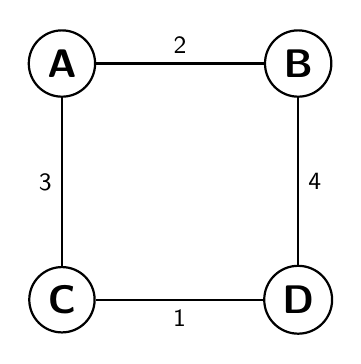
\begin{tikzpicture}[auto, node distance=3cm, thick, main node/.style={circle, draw, font=\sffamily\Large\bfseries}]
	\node[main node] (A) {A};
	\node[main node] (B) [right of=A] {B};
	\node[main node] (C) [below of=A] {C};
	\node[main node] (D) [below of=B] {D};
	\path[every node/.style={font=\sffamily\small}]
		(A) edge node [above] {2} (B)
		(B) edge node [right] {4} (D)
		(D) edge node [below] {1} (C)
		(C) edge node [left] {3} (A);
\end{tikzpicture}
\\
In this example, if we set $k = 2$, then the first $2$ edges chosen by Prim's algorithm will be edge $(A, B)$ and then edge $(A, C)$ with cost of $2 + 3 = 5$. However, the cheaper subgraph with just $2$ edges would be edge $(A, C)$ and then edge $(C, D)$ with cost of $3 + 1 = 4$.
\end{enumerate}


\newpage
\section*{2.  Uniqueness of Minimum Spanning Tree}
\begin{enumerate}[label=(\alph*)]
\item
In the graph below, there are multiple MSTs.
\\
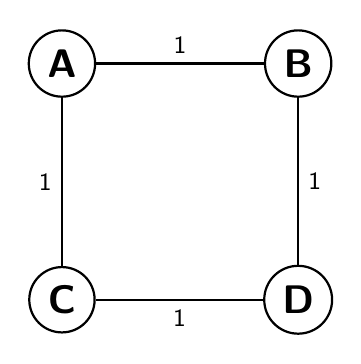
\begin{tikzpicture}[auto, node distance=3cm, thick, main node/.style={circle, draw, font=\sffamily\Large\bfseries}]
	\node[main node] (A) {A};
	\node[main node] (B) [right of=A] {B};
	\node[main node] (C) [below of=A] {C};
	\node[main node] (D) [below of=B] {D};
	\path[every node/.style={font=\sffamily\small}]
		(A) edge node [above] {1} (B)
		(B) edge node [right] {1} (D)
		(D) edge node [below] {1} (C)
		(C) edge node [left] {1} (A);
\end{tikzpicture}
\\
In this example, if we start from node $A$, then there are two MSTs: $A \rightarrow B \rightarrow D \rightarrow C$ and $A \rightarrow C \rightarrow D \rightarrow B$.

\item
The Cut Property was given to us as: Suppose edges $X$ are part of at least one MST of $G = (V, E)$. Pick any subset of nodes $S$ for which $X$ does not cross between $S$ and $V − S$, and let $e$ be the lightest edge across this partition. Then, $X \cup {e}$ is part of some MST. To prove the Unique Cut Property, I will start with the properties of MSTs and of $e$. If $e$ is the lightest edge across the partition and is unique, then if the MST contains $X$ then $X$ must contain $e$. This is because if a MST did not contain $e$ but instead included another cut, then it would not be a MST, which is a contradiction. The only way for it to be a MST without containing $e$ means that it can only have another cut of the same weight as $e$. However, this would mean that $e$ is no longer unique when $e$ is supposed to be unique.

\item
To prove this problem, I will need to prove that $E'$ forms a spanning tree implies that $G$ has a unique minimum spanning tree and that $G$ having a unique minimum spanning tree implies that $E'$ forms a spanning tree. To prove that $E'$ forms a spanning tree implies that $G$ has a unique minimum spanning tree, I will state that every graph $G$ has a MST and this MST is unique if it is the only one in the graph. So let us assume that this MST contains $E'$. The only way it would not be a unique MST is if there exists another MST of $G$ which does not contain exactly all the edges in $E'$. However, it is impossible for there to be a MST that does not contain all of $E'$. This is because if a MST does contain all the edges in $E'$ then there is an edge, $e_{alternate}$, that crosses the cut without being a member of $E'$. However, the cost of $e_{alternate} > (e \exists E')$. However then it isn't a MST then. To show that $G$ having a unique minimum spanning tree implies that $E'$ forms a spanning tree, I will assume that the MST is not unique, which I will call MST'. This means that there exists another MST that contains $E'$ that is different by differing by at least $1$ edge, which I will call MST''. This means that MST' has $e'$ while MST'' has $e''$. By the Unique Cut Property, the lightest edge between $e'$ and $e''$ would be in both MSTs so if we were to define $e'$ and $e''$ by the lighest edge to cross cut and incident to one of the nodes to which both edges are incident to, then we will notice that $e' = e''$. This means that the MST' and MST'' are the same so the MST that contains $E'$ must be unique.

\item
\begin{FourPartSolution}
\\
\begin{mainIdea}
\\
The main idea is to make a modification of Kruskal's algorithm to take advantage of Kruskal's algorithm being able to detect if an edge creates a cycle (with its find() function). This is helpful because if the edge that would have created a cycle is of the same weight as any of the weights in that almost-cycle, then there are multiple lightest edges in a cut.
\end{mainIdea}
\\
\begin{pseudocode}
\begin{lstlisting}
modifiedKruskal(G, w):
	for all u in V:
		makeset(u)
	X = {}
	sort the edges E by weight
	for all edges {u, v} in E, in increasing order of weight:
		if find(u) != find(v):
			add edge {u, v} to X
			union(u, v)
		else:
			if weight(edge{u, v}) == weight(e) for any e in find(u):
				return false
	return true
\end{lstlisting}
\end{pseudocode}
\begin{proofOfCorrectness}
\\
The pseudocode works because it just expands to Kruskal's algorithm by checking if the weight of an edge that would have created a cycle has the same weight as any of the weights in that almost-cycle. From part (c), we have shown that if the weight of an edge that would have created a cycle has the same weight as any of the weights in that almost-cycle, then there is not a unique MST. That is why the pseudocode will return false if that condition is met.
\end{proofOfCorrectness}
\\
\begin{runTime}
\\
$O((|V| + |E|) \log{|V|})$.
\end{runTime}
\\
\begin{justification}
\\
Since the pseudocode is just using normal Kruskal's algorithm with a conditional added to it, the run time is still the run time of Kruskal's algorithm, which is $O((|V| + |E|) \log{|V|})$.
\end{justification}
\end{FourPartSolution}
\end{enumerate}



\newpage
\section*{3. A Wizardry Party}
\begin{FourPartSolution}
\begin{mainIdea}
\\
Because you know the relative age of $y_i$ if you know that there is a DFS traversal between $x_i$ and $y_i$. So, as you learn more information at the party, you can create a graph. For example, if you learn that $x_i$ is $d_i$ years older than $y_i$, then you can create an edge between $x_i$ and $y_i$ with weight $d_i$. For this problem, the idea is to have a directed graph and the undirected version of the same graph. When running DFS, you consider the undirected graph path and add or subtract intermediate edges between $x_i$ and $y_i$ based on the direction of the traversal in the directed graph. After finding calculating the age between $x_i$ and $y_i$ you add an edge with the edge weight being the calculated age on the graphs to improve runtime on repeated calculations.
\end{mainIdea}

\begin{pseudocode}
\begin{lstlisting}
Graph G(V, E)
for i in timeSteps:
	if we are given x_i, y_i, d_i:
		add edge {x_i, y_i} with weight d_i to graph G:
	else:
		run DFS(G, x_i)
		if x_i.prenumber < y_i.prenumber and x_i.postnumber > y_i.postnumber:
			return weight of path and add to path
		else:
			return  "I don't know"
\end{lstlisting}
\end{pseudocode}
\begin{proofOfCorrectness}
\\
If there is a path between two nodes, then there are edges between the nodes. Furthermore, we are given the ages through the edges. When running DFS, we just use arithmetic to deduce the age between the two nodes.
\end{proofOfCorrectness}
\\
\begin{runTime}
\\
$O(m)$.
\end{runTime}

\begin{justification}
\\
When we add edges whenever calculating the relative edge, as $m$ approaches infinity, finding the number of relative edges for any pair of wizards will also approach $m$.
\end{justification}
\end{FourPartSolution}



\newpage
\section*{4. Arbitrage}
\begin{enumerate}[label=(\alph*)]
\item


\item


\end{enumerate}




\newpage
\section*{5. Premium Member}
\begin{FourPartSolution}
\begin{mainIdea}
\\

\end{mainIdea}

\begin{pseudocode}
\begin{lstlisting}

\end{lstlisting}
\end{pseudocode}
\begin{proofOfCorrectness}
\\

\end{proofOfCorrectness}
\\
\begin{runTime}
\\

\end{runTime}

\begin{justification}
\\

\end{justification}
\end{FourPartSolution}



\end{document}
